\section{Lebesgue Integration}

  Remember that Riemann integration is characterized by the approximation of step functions, which are the "building blocks" of Riemann integrable functions. To define the Lebesgue integral, we will start off with simple functions---which are a generalization of step functions. A function will be Lebesgue integrable if it can be approximated by these simple functions in some appropriate way. There are parallels between how we construct the Riemann and Lebesgue integral, namely that we can define the upper and lower integrals as the infimums and supremums of some set. However---while we were able to do this in ``one shot'' for the Riemann integral, the Lebesgue integral requires us to take intermediate steps. There are two ways that we can construct the Lebesgue integral. 
  \begin{enumerate}
    \item We define the integral for simple functions $\phi$ over finite measure. Since simple functions are made up of a linear combination of indicators, which are themselves bounded, the finite measure locks in the property that $\int \phi$ will be bounded. This allows us to take the integral of simple functions that have real-valued coefficients---both positive and negative---but is inherently limiting as we can't define the integral over infinite measures. With this, we can define the integral of bounded measurable functions using the lower and upper integrals. This is similar to the construction of the Riemann integral. Furthermore, if we want to define the general integral, we have to now restrict what we have built up into the nonnegative case---a bit unnatural. 

    \item We first define the integral for \textit{nonnegative} simple functions $\phi$ over any measure. We are sacrificing the ability to integrate negative simple functions early on, but this doesn't matter since we will split functions into a positive and negative part anyways. The true advantage of doing this is that we gain the ability to define integrals for infinite measures. This allows us to define for positive (possibly unbounded) measurable functions, and finally when we define the general Lebesgue integral, we deal with the $\infty - \infty$ problem by defining it only if at least one of the positive or negative integrals are finite. 
  \end{enumerate}

  I personally think the second way is superior, since in the end we can define integrals over infinite measure. Furthermore, since we are only working with positive functions, we only need to define the lower integral rather than checking to see if the lower and upper integrals coincide. 

  As we redefine these integrals over and over (sort of like method overriding), we really want to preserve three properties of the integral. 
  \begin{enumerate}
    \item Linearity. 
      \begin{equation}
        \int_E (\alpha f + \beta g) = \alpha \int_E f + \beta \int_E g 
      \end{equation}

    \item Monotonicity 
      \begin{equation}
        f \leq g \implies \int_E f \leq \int_E g 
      \end{equation}

    \item Additivity. 
      \begin{equation}
        A, B \text{ disjoint, measurable, and } E = A \cup B \implies \int_E f = \int_A f + \int_B f
      \end{equation}
  \end{enumerate}

\subsection{Simple Functions} 

  We will use $\phi, \varphi, \psi$ to denote simple functions. 

  \begin{definition}[Lebesgue Integral of Simple Functions over Finite Measure]
    Suppose $\phi = \sum_{k=1}^n a_k \chi_{E_k}: E \subset \mathbb{R} \to \mathbb{R}$ with $a_k \in \mathbb{R}$. 
    \begin{enumerate}
      \item If $m(E) < +\infty$, then we can define the integral which is guaranteed to be a finite number.  
      \begin{equation}
        \int_E \phi \coloneqq \sum_{k=1}^n a_k m(E_k)
      \end{equation} 

      \item If $a_k \geq 0$, we define the integral which lives in $\mathbb{R} \cup \{+\infty\}$.\footnote{As we have stated before, we could also define the Lebesgue integral of simple functions by letting $a_k$ takes values in $\mathbb{R}$. But then, we might have a case where $E = A \sqcup B$, with $m(A) = +\infty, m(B) = +\infty$, and $\phi = \chi_{A} - 2 \chi_{B} \implies \int_E \phi = \infty - \infty$. To prevent this from happening, some authors add the assumption that $m(E) < +\infty$, and I cover this case to make it as comprehensive as possible. }
      \begin{equation}
        \int_E \phi \coloneqq \sum_{k=1}^n a_k m(E_k)
      \end{equation} 
    \end{enumerate}
    This is well defined for any representation of $\phi$\footnote{We need this since the coefficients need not be unique. For example, we can write $1 \cdot \chi_{[0, 1]} + 1 \cdot \chi_{[0.5, 1]} = 1 \cdot \chi_{[0, 0.5]} + 2 \cdot \chi_{[0.5, 1]}$. If the $E_i$'s are disjoint, then this decomposition is unique and is called the \textbf{standard representation} of $\phi$. } 
  \end{definition} 
  \begin{proof}
    It is clear that the two definitions coincide if $m(E) < +\infty$ and $a_k \geq 0$ is true; it is the same formula.  
  \end{proof} 

  For bounded functions, we will temporarily focus on the first definition, and for general functions, we rely on the second definition. 

  \begin{theorem}[Integral Properties for Simple Functions over Finite Measure]
    Suppose $\phi, \psi: E \subset \mathbb{R} \to \mathbb{R}$ are simple with $m(E) < +\infty$. Then, the following properties hold. 
    \begin{enumerate}
      \item Linearity. For $\alpha, \beta \in \mathbb{R}$, 
        \begin{equation}
          \int_E (\alpha \phi + \beta \psi) = \alpha \int_E \phi + \beta \int_E \psi
        \end{equation}

      \item Monotonicity. 
        \begin{equation}
          \phi \leq \psi \implies \int_E \phi \leq \int_E \psi 
        \end{equation}

      \item Additivity. If $A, B$ are disjoint, measurable, and $E = A \cup B$, then 
        \begin{equation}
          \int_E \phi = \int_A \phi + \int_B \phi
        \end{equation}
    \end{enumerate}
  \end{theorem}
  \begin{proof}
    Listed. 
    \begin{enumerate}
      \item We can subdivide sets s.t. $\phi$ and $\psi$ can be rewritten using the same finite family of sets $A_k$. 
      \item We can use (1) to rewrite 
        \begin{equation}
          \int_E \psi - \int_E \phi = \int \underbrace{(\psi - \phi)}_{\geq 0 \forall x} \geq 0
        \end{equation}

      \item Trivial by definition of simple functions. 
    \end{enumerate}
  \end{proof}

  \begin{example}[Step Function as Simple Function]
    For $a, b \in \mathbb{R}$, with $a < b$, let $f: [a, b] \longrightarrow \mathbb{R}$ be a step function. That is, there exists a partition $a = x_0 < x_1 < \ldots < x_n = b$ and constants $c_1, c_2, \ldots, c_n \in \mathbb{R}$ s.t. $f(x) = c_i$ for all $x \in (x_{i-1}, x_i)$ and each $i = 1, \ldots, n$. Then, $f$ is equal to the following simple function, taken over all open intervals and the points $x_j$ at the boundary of each interval. 
    \begin{equation}
      f = \sum_{i=1}^n c_i \chi_{(x_{i-1}, x_i)} + \sum_{j=0}^n f(x_j) \chi_{\{x_j\}}
    \end{equation}
    If we ignore the behavior of $f$ on the partition points $x_j$'s, then $f$ agrees almost everywhere with the simple function 
    \begin{equation}
      \sum_{i=1}^n c_i \chi_{(x_{i-1}, x_i)}
    \end{equation}
  \end{example} 

\subsection{Bounded Functions} 

  This isn't the most popular way to define Lebesgue integrability, but I'd like to compare it to Riemann integral. First, note that a Riemann integral 

  \begin{definition}[Lower, Upper Lebesgue Integral]
    Let $f: E \subset \mathbb{R} \to \mathbb{R}$ be bounded, with $m(E) < +\infty$. Then, the \textbf{upper and lower Lebesgue integrals} are defined 
    \begin{equation}
      \overline{L} f \coloneqq \inf_{\phi} \bigg\{ \int \phi \; \bigg| \; f \leq \phi, \phi \text{ simple} \bigg\}, \qquad \underline{L} f \coloneqq \sup_{\phi} \bigg\{ \int \phi \; \bigg| \; \phi \leq f, \phi \text{ simple} \bigg\}
    \end{equation}
    If the upper and lower Lebesgue integrals are equal, then $f$ is said to be \textbf{Lebesgue integrable}.
  \end{definition}

  This is exactly the same form as that of \hyperref[real-def:riemann-integral]{Riemann integration}, notably that $f$ must be bounded and we define integrability as the equivalence of the upper and lower integrals. The fact that $m(E)$ is finite is realized implicitly with partitions, though in this sense it's more similar to the Riemann-Stieltjes integral. From this, it's pretty easy to intuit that the Lebesgue integral agrees with the Riemann integral for step functions. Let $c_1, \ldots, c_n \in [0, \infty)$ and $a = x_0 < x_1 < \ldots < x_n = b$ be a partition. Let $f: [a, b] \longrightarrow [0, \infty]$ be a step function taking the value $c_i$ on the interval $(x_{i-1}, x_i)$ for $i = 1, \ldots, n$. Then the Riemann integral of $f$ is simply 
  \begin{equation}
    \int f(x) \,dx = \sum_{i=1}^n c_k |x_i - x_{i-1}|
  \end{equation}
  The Lebesgue integral is 
  \begin{equation}
    \int f \, d \mu = \sum_{i=1}^n c_i \mu((x_{i-1}, x_i)) + \sum_{j=0}^n f(x_j) \mu(\{x_j\}) = \sum_{i=1}^n c_k |x_i - x_{i-1}|
  \end{equation}
  which agrees with the Riemann integral. In the Riemann integral, we write $dx$ to indicate the variable that is being integrated over, but in the Lebesgue integral, we write $d \mu$, the measure which we are integrating over. We make this more rigorous in the following theorem.  

  \begin{theorem}[Riemann Integrability Implies Lebesgue Integrability]
    If $f$ is Riemann integrable, then it is Lebesgue integrable. 
  \end{theorem}
  \begin{proof}
    Recall that $f$ is Riemann integrable if 
    \begin{equation}
      \sup_P L(P, f) = \inf_P U(P, f)
    \end{equation} 
    for a partition $P$. But for any $L(P, f)$ (or $U(P, f)$), there exist simple $\phi$ (or $\psi$) s.t. 
    \begin{equation}
      \int_E \phi = L(P, f), \qquad \bigg( \int_E \psi = U(P, f) \bigg)
    \end{equation}
    So, 
    \begin{equation}
      \sup_P L(P, f) \leq \underline{L} f \leq \overline{L} f \leq \inf_P U(P, f) 
    \end{equation}
    where the first and third inequalities we just showed, and the middle inequality $\underline{L} f \leq \overline{L} f$ comes from monotonicity. So if the $\inf = \sup$, then $\underline{L} f = \overline{L} f$ has nowhere to go. 
  \end{proof} 

  However, the converse is not true. 

  \begin{example}[Lebesgue Integrable but Not Riemann Integrable]
    Consider the simple function (consisting of one characteristic function) $\chi_{\mathbb{Q} \cap [0, 1]}$. $\mathbb{Q} \cap [0, 1]$ is a Lebesgue measurable set of $\mathbb{R}$, and we have $\chi_{\mathbb{Q} \cap [0, 1]} \geq 0$, so its Lebesgue integral is given by the above definition: 
    \begin{equation}
      \int_{\mathbb{R}} \chi_{\mathbb{Q} \cap [0, 1]} \, d\lambda = 1 \cdot \lambda(\mathbb{Q} \cap [0, 1]) = 0
    \end{equation}
  \end{example} 

  Remember that \hyperref[real-thm:continuous-riemann]{continuous functions are Riemann integrable}. There is indeed an analogous result between measurable functions and Lebesgue-integrable functions. 

  \begin{theorem}[Measurable Functions are Lebesgue Integrable]
    Let $f: E \subset \mathbb{R} \to \mathbb{R}$ be measurable, bounded with $m(E) < +\infty$. Then, $f$ is Lebesgue integrable. 
  \end{theorem}
  \begin{proof}
    We prove that $\forall n$, $\exists$ a simple $\phi_n, \psi_n$ s.t. $\phi_n \leq f \leq \psi_n$  and $\psi_n - \phi_n < 1/n$. Then, 
    \begin{equation}
      \overline{L} f - \underline{L} f \leq \int \psi_n - \int \phi_n \leq \frac{1}{n} m(E)
    \end{equation}
    So take $n \to \infty$. 
  \end{proof}

  Now, we have a much larger class of functions we can integrate. It turns out that there is an iff condition for Lebesgue integrability. 

  \begin{theorem}[Lebesgue Integrable iff Set of Discontinuities have Measure 0]
    A function $f: E \subset \mathbb{R}$ is Lebesgue integrable iff $f$ is continuous almost everywhere. 
  \end{theorem}
  \begin{proof}
    
  \end{proof} 

  To prove additivity, we'll need a specific lemma. 

  \begin{lemma}[]
    Let $f: E \subset \mathbb{R} \to \mathbb{R}$ be measurable, bounded with $m(E) < +\infty$, and $A \subset E$ measurable. Then, 
    \begin{equation}
      \int_E f \cdot \chi_A = \int_A f
    \end{equation}
  \end{lemma}
  \begin{proof}
    
  \end{proof}

  \begin{theorem}[Integral Properties for Bounded Measurable Functions over Finite Measure]
    Suppose $f, g: E \subset \mathbb{R} \to \mathbb{R}$ are bounded and measurable with $m(E) < +\infty$. Then, the following properties hold. 
    \begin{enumerate}
      \item Linearity. For $\alpha, \beta \in \mathbb{R}$, 
        \begin{equation}
          \int_E (\alpha f + \beta g) = \alpha \int_E f + \beta \int_E g
        \end{equation} 

      \item Monotonicity. 
        \begin{equation}
          f \leq g \implies \int_E f \leq \int_E g
        \end{equation}

      \item Additivity. If $A \subset E$ is measurable $B = A \setminus E$, then 
        \begin{equation}
          \int_E f  = \int_A f + \int_B f
        \end{equation}
    \end{enumerate}
  \end{theorem}
  \begin{proof} 
    Listed. 
    \begin{enumerate}
      \item For scalar multiplication, we just use $\alpha \phi, \alpha \psi$ in the simple function approximation. Now for the sums of functions, we can see that 
        \begin{align}
          f \leq \psi_1, g \leq \psi_2 & \implies f + g \leq \psi_1 + \psi_2 \implies \int (f + g) \leq \int f + \int g \\ 
          f \geq \psi_1, g \geq \psi_2 & \implies f + g \geq \psi_1 + \psi_2 \implies \int (f + g) \geq \int f + \int g \\ 
        \end{align} 
        and by taking the limit as the simple functions approach $f, g$, we get equality. 
      \item 
      \item We can define $f_1 = f \cdot \chi_A, f_2 = f \cdot \chi_B$. $f_1, f_2$ are measurable and bounded (as the product of measurable functions) implying that 
        \begin{equation}
          \int_E f = \int_E (f_1 + f_2) = \int_E f_1 + \int_E f_2 = \int_E f \cdot \chi_A + \int_E f \cdot \chi_B = \int_A f + \int_B f
        \end{equation}
        where the final equality follows from the lemma. 
    \end{enumerate}
  \end{proof} 

  \begin{corollary}[]
    Suppose $f: E \subset \mathbb{R} \to \mathbb{R}$ is bounded and measurable. Then 
    \begin{equation}
      \bigg| \int_E f \bigg| \leq \int_E |f| 
    \end{equation}
  \end{corollary} 
  \begin{proof}
    We know $-|f| \leq f \leq |f|$. By monotonicity, we have 
    \begin{equation}
      \int -|f| \leq \int f \leq \int |f|
    \end{equation}
  \end{proof} 

  The next theorem is sort of like transferring convergence of functions to that of integrals. This results shouldn't be surprisingly since uniform convergence is so strong.  

  \begin{theorem}[Uniform Convergence Implies Convergence of Integrals]
    Suppose $f_n$ are bounded, measurable, and $f_n \to f$ uniformly on $E$ with $m(E) < +\infty$. Then, 
    \begin{equation}
      \int_E f_n \to \int_E f
    \end{equation}
  \end{theorem} 
  \begin{proof} 
    Since $f$ is bounded, there exists $N \in \mathbb{N}$ s.t. $\| f_N - f \|_{\infty} \leq 1$. Then, by reverse triangle inequality (?), $\|f\|_\infty \leq \|f_N\|_\infty + 1$. Also, $f$ is measurable as the limit of $f_N$. Given $\epsilon > 0$, find $N_1$ s.t. $\forall n \geq N_1$, 
    \begin{align}
      \|f_n - f\|_\infty \leq \frac{\epsilon}{m(E)} \implies  \bigg| \int f - \int f_n \bigg| = \bigg| \int_E (f - f_n) \bigg| \leq \int_E |f - f_n| \leq \frac{\epsilon}{m(E)} \cdot m(E) = \epsilon
    \end{align}
  \end{proof}

  Naturally we might see if this results holds with weaker assumptions. Unfortunately, this is not true for pointwise convergence. 

  \begin{example}[Integrals Don't Converge Under Pointwise Convergence]
    Let $f_n (x) = n \cdot \chi_{[0, 1/n]} (x)$, so $f_n (x) \to 0$ a.e. in $[0, 1]$ but $\int f_n (x) = 1$ for all $n \in \mathbb{N}$. 
  \end{example}

  But not all hope is lost. This is where the key theorems of measure theory comes in. The following theorem is more general, since uniform convergence implies uniformly bounded, but it isn't used in practice as much (according to Kiselev). 

  \begin{theorem}[Bounded Convergence Theorem]
    Suppose $f_n$ are measurable, uniformly bounded.\footnote{$\|f_n\|_\infty \leq M < \infty$} Suppose $f_n \to f$ pointwise on $E$, with $m(E) < \infty$. Then, 
    \begin{equation}
      \int_E f_n \to \int_E f
    \end{equation}
  \end{theorem}
  \begin{proof}
    $f$ is bounded because $f_n$ are uniformly bounded, and it is measurable since it's a limit of measurable functions. Fix $\epsilon > 0$. by Egoroff, $\exists F \subset E$ s.t. $f_n \to f$ uniformly on $F$, and $m(E \setminus F) \leq \frac{\epsilon}{4M}$. Then, 
    \begin{equation}
      \bigg| \int_E f - \int_E f_n \bigg| \leq \int_E |f - f_n| = \int_F |f - f_n| + \int_{E \setminus F} |f - f_n| 
    \end{equation}
    For the first term, $\exists N \in \mathbb{N}$ s.t. if $n \geq N$, then $|f_n (x) - f(x)| \leq \frac{\epsilon}{2 m(F)} \leq \epsilon{2}$ for all $x \in F$. For the second term, we can bound this by $2M \cdot \frac{\epsilon}{4M} \leq \frac{\epsilon}{2}$. Therefore, the whole expression $\leq \frac{\epsilon}{2} + \frac{\epsilon}{2} = \epsilon$. 
  \end{proof}

  However, this assumption is still too strong for convergence and is therefore not used much in practice unlike other theorems (e.g. monotone convergence theorem and dominated convergence theorem). One nice part is that it works for unbounded functions, which is good since working with bounded functions is not the most natural assumption to have in practice. This is why we will step back and reconstruct the Lebesgue integral using positive---and possibly unbounded---simple functions (1st definition). 

\subsection{Positive Functions}

  If the $A_i$'s are just intervals in $\mathbb{R}$, then $\phi$ reduces to a step function. But the entire problem with intervals is that they are too coarse. We can't work with them, so we generalize them to all measurable sets in $(X, \mathcal{A})$. The Riemann integral is built on an approximation scheme of a function, which we usually want to be continuous to satisfy this approximation, and so, if we want to build an approximation scheme for Lebesgue integrals, we want a similar scheme, i.e. if we take a sequence of simple measurable functions, I can get arbitrarily close to any measurable function $f$. This is exactly what we show below. 

  \begin{theorem}
    If $f: (X, \mathcal{A}) \longrightarrow [0, \infty]$ is measurable, there are simple measurable functions $f_k : (X, \mathcal{A}) \longrightarrow [0, \infty)$ s.t. 
    \begin{equation}
      f_k \leq f_{k+1} \text{ and } f = \lim_{k \rightarrow \infty} f_k
    \end{equation}
    where the inequalities and limits are pointwise. 
  \end{theorem}
  \begin{proof}
    We give a general picture of this proof for a function $f: \mathbb{R} \longrightarrow [0, \infty]$. We can first divide the codomain of the graph below into segments of $t = 1, 2, \ldots$, and take the preimage of all these units under $f$ to get $f_1$. More specifically, $A_1^t = f^{-1} ([t, \infty])$ for all $t$. By measurability of $f$, $A_1^t$ is measurable, and we can assign $f_1 = \chi_{A^1_1} + \chi_{A_1^2} \leq f$. 
    \begin{center}
        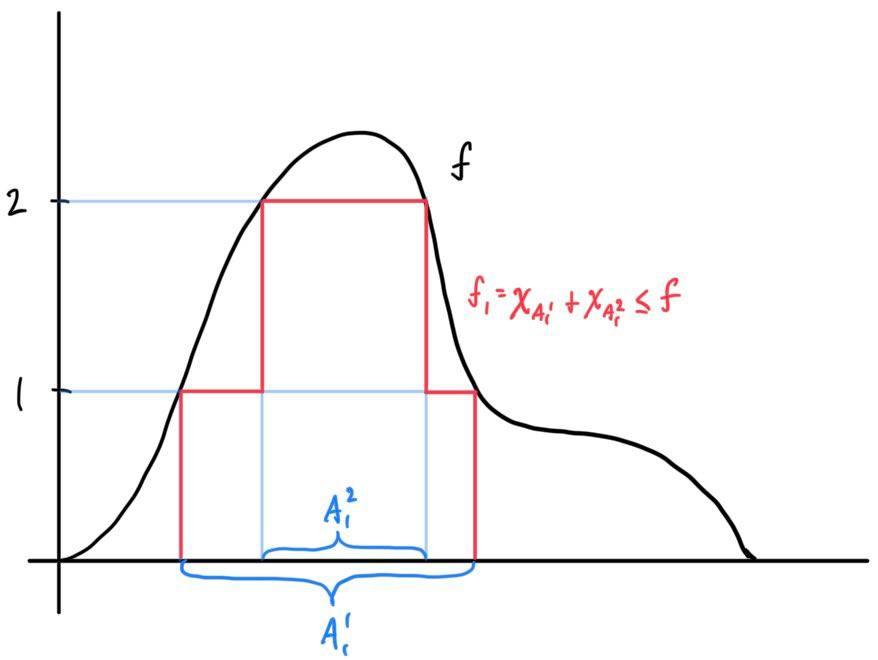
\includegraphics[scale=0.23]{img/Lebesgue_1.jpg}
    \end{center}
    Doing this again with finer subintervals of the codomain gives us, with $f_2 = \chi_{A_2^1} + \chi_{A_2^2} + \chi_{A_2^3} + \chi_{A_2^4} \leq f$. 
    \begin{center}
        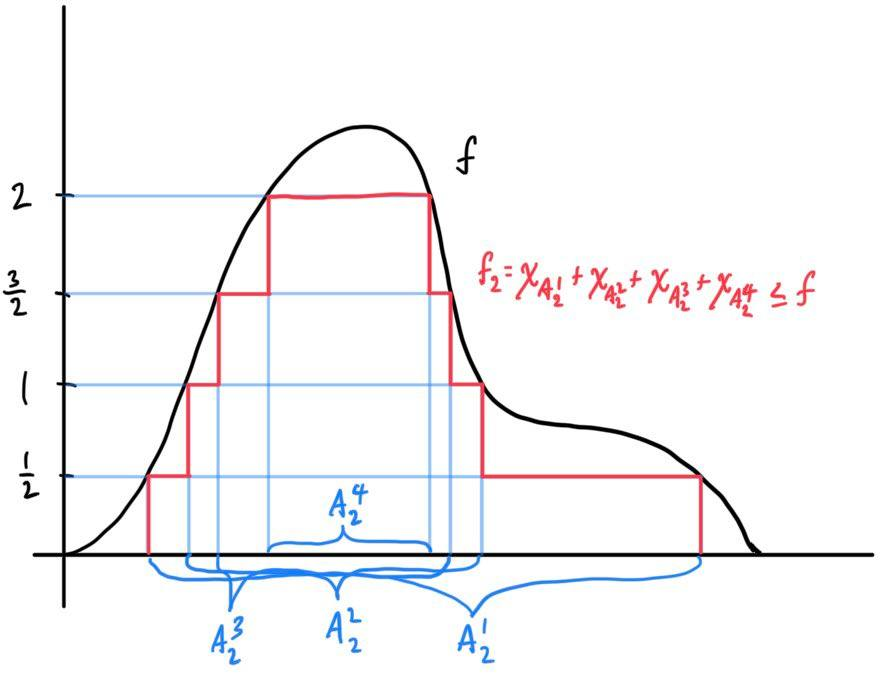
\includegraphics[scale=0.23]{img/Lebesgue_2.jpg}
    \end{center}
    and in general, we have $f_k = \sum_{j=1}^\infty \frac{1}{2^{k-1}} \chi_{A^j_k}$. But we said a simple function is a \textit{finite} sum, and if $\infty$ is in the range of $f$, then this becomes a problem. We can quickly fix this by just truncating the summation at a certain point in the codomain ($f_1$ only considers intervals up to $1$, $f_2$ up to $2$ and so on), ultimately giving us 
    \begin{equation}
      f_k = \sum_{j=1}^{k 2^{k-1}} \frac{1}{2^{k-1}} \chi_{A^j_k} 
    \end{equation}
  \end{proof}

  Finally, we can learn how to integrate. We require the positiveness condition on $f$ below because our previous theorem on approximating arbitrary functions with simple measurable functions $f_k$ requires that it be positive, too. 

\subsection{Positive Measurable Functions} 

  The next natural step to generalize Lebesgue integral is to look at unbounded functions and/or infinite measures. In order to do this, we must start off by stepping back into only nonnegative functions first.

  Unlike Riemann integration and Lebesgue integration of signed bounded functions, which looks at both the supremum and infimum of integrals of simple functions, Lebesgue integration of positive only looks at the supremum, given that $f$ is nonnegative, so for all these $f$, the Lebesgue integral always exists. 

  \begin{definition}[Lebesgue Integral on Positive Measurable Functions]
    Let $f: E \subset \mathbb{R} \to \mathbb{R}$ satisfy $f \geq 0$, with $E$ measurable (but not necessarily that $m(E) < +\infty$). Then, the \textbf{Lebesgue integral} is defined 
    \begin{align}
      \int_E f & \coloneqq \sup \bigg\{ \int_E h \; \bigg| \; 0 \leq h \leq f, h \text{ measurable, bounded} \bigg\} \\ 
               & = \sup \bigg\{ \int_E \phi \; \bigg| \; 0 \leq \phi \leq f, \phi \text{ simple} \bigg\}
    \end{align}
  \end{definition}
  \begin{proof}
    The only thing to show is that it suffices to check for simple functions only, so all we have to do is check the latter form. 
  \end{proof} 

  \begin{lemma}[Chebyshev]
    Suppose $f: E \subset \mathbb{R} \to \mathbb{R}$, $f \geq 0$, and $f$ is measurable. Then for all $\alpha > 0$,\footnote{In probability, this refers to a bound on the variance of a random variable, but in analysis, it seems to be a more general result of the bounds of form $\int |f|^p$.} 
    \begin{equation}
      m( \{ x \in E \mid f(x) \geq \alpha\}) \leq \frac{1}{\alpha} \int_E f 
    \end{equation}
  \end{lemma}
  \begin{proof}
    Let us call the set on the LHS $E_\alpha$. Then, $E_\alpha$ is measurable and define $\phi(x) = \alpha \chi_{E_\alpha} (x)$. Then, $\phi(x) \leq f(x)$, and so 
    \begin{equation}
      \int f \geq \int \phi = \alpha m(E_\alpha)
    \end{equation}
  \end{proof}

  \begin{theorem}[Vanishing Integral iff a.e. Vanishing Function]
    Suppose $f \geq 0$ on $E$. Then, 
    \begin{equation}
      \int_E f = 0 \iff f = 0 \text{ a.e. on } E
    \end{equation}
  \end{theorem}
  \begin{proof}
    We prove bidirectionally. 
    \begin{enumerate}
      \item $(\rightarrow)$. By Chebyshev, we see that 
        \begin{equation}
          m(\underbrace{\{ x \in E \mid f(x) \geq 1/n \}}_{E_n}) \leq n \int f = 0 
        \end{equation}
        for all $n \in \mathbb{N}$. But $\{x \in E \mid f(x) > 0\} = \cup_{n=1}^\infty E_n$. By countable additivity, $m(\{x \in E \mid f(x) > 0\}) = 0$. 

      \item $(\leftarrow)$. Since $f = 0$ a.e., any $0 \leq \phi \leq f$---$\phi$ simple---will satisfy $m(\{x \in E \mid \phi(x) = 0 \}) = 0$, but it will never get off $0$. Therefore, $\int_E \phi = 0$. 
    \end{enumerate}
  \end{proof}

  \begin{theorem}[Integral Properties for Nonnegative Measurable Functions]
    Suppose nonnegative $f, g: E \subset \mathbb{R} \to \mathbb{R}$ are measurable. Then, 
    \begin{enumerate}
      \item Linearity. For all $\alpha, \beta \geq 0$,\footnote{Note that we have $\geq 0$ since we are dealing with positive functions!} 
        \begin{equation}
          \int_E (\alpha f + \beta g) = \alpha \int f + \beta \int g 
        \end{equation}

      \item Monotonicity. 
        \begin{equation}
          f \leq g \implies \int f \leq \int g 
        \end{equation}

      \item Additivity. If $A, B$ are disjoint with $E = A \cup B$, then 
        \begin{equation}
          \int_E f = \int_A f + \int_B f
        \end{equation}
    \end{enumerate}
  \end{theorem}
  \begin{proof}
    Listed. 
    \begin{enumerate}
      \item We can easily show $\int \alpha f = \alpha \int f$ simply by multiplying the simple functions $\phi$ by $\alpha$. For integrals of sums of functions, we show the following. 
      \begin{enumerate}
        \item $\int f + \int g \leq \int (f + g)$. Since given simple $\phi_1, \phi_2$ with $\phi_1 \leq f, \phi_2 \leq g$, we have $\phi_1 + \phi_2 \leq f + g$, and so by taking the supremum, we have the bound. 

        \item $\int f + \int g \geq \int (f + g)$. Suppose $h$ is simple s.t. $0 \leq h \leq f + g$. Define\footnote{Intuitively, we are trying to split the $f + g$ into $\ell$ and $k$, such that $\ell + k = h \leq f + g$.} 
          \begin{equation}
            \ell \coloneqq \min\{h, f\}, \qquad k \coloneqq h - \ell
          \end{equation}
          Note that $\ell, k$ are both measurable. Furthermore, $\ell$ is at most $h$ (which is simple) and so is bounded, and $k$ is also bounded since it is bounded $h$ minus some nonnegative $\ell$ that is at most $h$. Therefore, we invoke our previous definition of the Lebesgue integral for bounded functions to get 
          \begin{equation}
            \int k + \int \ell = \int h
          \end{equation}
          Since $\ell \leq f$ and $k = h - \ell \leq g$, by monotonicity we have $\int k \leq \int g$ and $\int \ell \leq \int f$. Substituting this in gives 
          \begin{equation}
            \int h \leq \int f + \int g \implies \int (f + g) = \sup_h \int h \leq \int f + \int g
          \end{equation}
        \end{enumerate}
      \item Direct. 
      \item 
    \end{enumerate}
  \end{proof}

  We know that the integral doesn't behave well under weak kinds of convergence, e.g. pointwise or a.e. The following theorem gives us a slightly stronger assumption. 

  \begin{theorem}[Monotone Convergene Theorem (MCT)]
    Given a nondecreasing sequence of nonnegative measurable functions $f_1 \leq f_2 \leq f_3 \leq \ldots : X \longrightarrow [0, \infty]$, its limit $\lim_{k \rightarrow \infty} f_k$ always exists (since $f_k$ is nondecreasing), is measurable, and 
    \begin{equation}
      \int \lim_{k \rightarrow \infty} f_k \, d\mu = \lim_{k \rightarrow \infty} \int f_k \, d\mu
    \end{equation}
  \end{theorem}
  \begin{proof}
    Suppose $\lim_{n \to \infty} \int f_n = \alpha$ (could be infinity), $f(x) \geq f_n (x)$ for all $x, n$, so $\int f \geq \alpha$. Consider $0 \leq \phi \leq f$, $\phi$ simple. Take $0 < c < 1$\footnote{We introduce the $c$ because we can then claim that the union of $E_n$ is $E$.} and define 
    \begin{equation}
      E_n \{x \mid f_n (x) \geq c \phi(x) \} 
    \end{equation} 
    Then, the $E_n$ are increasing and $\cup_{n=1}^\infty E_n = E$.\footnote{This may not be true is $c = 1$.} Observe that 
    \begin{equation}
      \int_{E_n} f_n \geq c \int_{E_n} \phi 
    \end{equation}
    Suppose that $\phi (x) = \sum_{k=1}^M a_k \chi_{F_k} (x)$. Then, 
    \begin{equation}
      \int_{E_n} f = \sum_{k=1}^M a_k m(F_k \cap E_n) \to \sum_{k=1}^M a_k m(F_k) = \int_E \phi \text{ as } n \to +\infty
    \end{equation} 
    Therefore, 
    \begin{equation}
      \lim_{n \to \infty} \int_E f_n \geq c \int_E \phi \forall c < 1 \implies \text{ also true for } c = 1
    \end{equation}
    Since $\phi \leq f$ is arbitrary, we get $\lim_{n \to \infty} \int f_n \geq \int f $. 
  \end{proof}

  This allows us to integrate the limit of nice functions $f_k$ by integrating these $f_k$ first and then finding what the values converge to. The huge problem with Riemann integrals is that this theorem doesn't hold, but it is the case for Lebesgue integration. In practice, the MCT is not as useful, but the following is. 

  \begin{lemma}[Fatau's Lemma]
    Suppose $f_n \geq 0$ and it converges to $f$. Then, 
    \begin{equation}
      \int_E \liminf{f_n} \leq \liminf \int_E f_n
    \end{equation}
  \end{lemma}
  \begin{proof}
    Define $g_k (x) = \int_{j \geq k} f_j (x)$. Note that $g_k (x) \leq f_k (x)$ by definition, and $g_k (x)$ is increasing. Since by definition $\lim_{k \to \infty} g_k (x) = \liminf f_k (x)$, by MCT, 
    \begin{equation}
      \lim_{k \to \infty} \int_E g_k = \int \liminf f_k 
    \end{equation}
    But since $\int g_k \leq \int f_k$ for all $k$, 
    \begin{equation}
      \liminf \int f_k \geq \int \liminf f_k 
    \end{equation}
  \end{proof}

  Note that equality does not have to hold. For example, take $f_n (x) = \chi_{[n, n+1]} (x)$. 

  \begin{definition}[Lebesgue Integrability]
    A positive measurable function $f$ is \textbf{Lebesgue integrable} if $\int f < +\infty$. 
  \end{definition}

  \begin{theorem}[]
    If $f$ is integrable on $E$, then $f(x) < +\infty$ a.e. on $E$. 
  \end{theorem}
  \begin{proof}
    By Chebyshev, 
    \begin{equation}
      m( \{x \in E \mid f(x) \geq n \}) \leq \frac{1}{n} \int_E f 
    \end{equation}
    As $n \to \infty$, the LHD is bounded above by all $\epsilon > 0$. 
    \begin{equation}
      m( \{x \in E \mid f(x) = \infty \}) = m \bigg( \bigcap_{n=1}^\infty E_n \bigg)
    \end{equation}
  \end{proof} 

  Here is a variant of MCT. 

  \begin{lemma}[Levi's Lemma] 
    Suppose $f_n \geq 0$ is increasing and $\int_E f_n \leq M$ for all $n$. Then, 
    \begin{enumerate}
      \item $f(x) = \lim_{n \to \infty} f_n (x)$ is integrable, and 
      \item $\int f \leq M$. 
    \end{enumerate}
  \end{lemma}
  \begin{proof}
    By MCT, $\int_E f_n \to \int_E f$. 
  \end{proof} 

\subsection{Lebesgue Integral for Signed Functions} 

  \begin{definition}[Lebesgue Integral for Signed Functions]
    Given $f: E \subset \mathbb{R} \to \mathbb{R} \cup \{\pm \infty\}$, let us write 
    \begin{equation}
      f = f^+ - f^-, \qquad f^+ \coloneqq \max \{0, f\}, f^- \coloneqq \max\{-f, 0\}
    \end{equation}
    $f$ is \textbf{Lebesgue integrable} iff $f^+$ and $f^-$ and we define the \textbf{Lebesgue integral} of $f$ as 
    \begin{equation}
      \int f \coloneqq \int f^+ - \int f^- 
    \end{equation}
    given that at least one of these integrals is finite. If one is infinite and the other is finite, then we can call it infinite. If we have \textit{both} infinite integrals, then the integral doesn't exist. 
  \end{definition} 

  If $f^+, f^-$ are Lebesgue integrable, then it can only be $\pm \infty$ on a set of measure $0$, so it generally won't affect anything. Also, there is a difference between the \textit{existence} of the integral and a function \textit{being} Riemann-integrable. 

  Since $|f| = f^+ + f^-$, $f$ is also Lebesgue integrable if 
  \begin{equation}
    \int |f| \, d\mu < \infty 
  \end{equation}
  since by triangle inequality, we have 
  \begin{equation}
    \bigg| \int f \, d\mu \bigg| \leq \int |f| \, d \mu
  \end{equation}

  \begin{theorem}
    $f^\pm$ integrable iff $|f|$ integrable. 
  \end{theorem}
  \begin{proof}
    $|f| = f^+ + f^-$. 
  \end{proof}

  \begin{theorem}[Integral Properties of Signed Measurable Functions]
    Suppose $f, g : E \subset \mathbb{R} \to \mathbb{R}$ are measurable. Then, 
    \begin{enumerate}
      \item Linearity. For all $\alpha, \beta \in \mathbb{R}$, 
        \begin{equation}
          \int_E (\alpha f + \beta g) = \alpha \int f + \beta \int g
        \end{equation}

      \item Monotonicity. 
        \begin{equation}
          f \leq g \implies \int f \leq \int g
        \end{equation}

      \item Additivity. If $A, B$ are disjoint with $E = A \cup B$, then 
        \begin{equation}
          \int_E f = \int_A f + \int_B f
        \end{equation}
    \end{enumerate}
  \end{theorem} 
  \begin{proof}
    Listed. As always, linearity is nontrivial. 
    \begin{enumerate}
      \item For scalar multiplication, we divide into 2 cases. 
        \begin{enumerate}
          \item $\alpha > 0$. Then, $(\alpha f)^+ = \alpha f^+$ and $(\alpha f)^- = \alpha f^-$, so 
            \begin{equation}
              \int (\alpha f) = \int \alpha f^+ - \int \alpha f^- = \alpha \int f
            \end{equation}

          \item $\alpha < 0$. Then, $(\alpha f)^+ = - \alpha f^+$ and $(\alpha f)^- = \alpha f^+$, so 
            \begin{equation}
              \int (\alpha f) = \int -\alpha f^- + \int \alpha f^+ = \alpha \bigg( \int f^+ - \int f^- \bigg) = \alpha \int f
            \end{equation}
        \end{enumerate}
      \item For addition, note that $|f + g| \leq |f| + |g|$, so it is integrable. So 
        \begin{equation}
          \int (f + g) = \int (f + g)^+ - \int (f + g)^- 
        \end{equation}
        Now observe that 
        \begin{align}
          (f + g)^+ - (f + g)^- & = f + g = f^+ + g^+ - f^- - g^- \\ 
          (f + g)^+ + f^- + g^- & = (f + g)^- + f^+ + g^+ 
        \end{align}
        Since it is nonnegative, our previous properties of linearity holds, and then we can just rearrange. 
      \item 
      \item 
    \end{enumerate}
  \end{proof}

  \begin{definition}[Normed Vector Space of Lebesgue Integrable Functions]
    The set of all functions $f: (X, \mathcal{A}, \mu) \longrightarrow \mathbb{R}$ that are Lebesgue integrable is denoted $\mathcal{L}^1(X, \mathcal{A}, \mu; \mathbb{R})$, or for short $\mathcal{L}^1(X, \mathcal{A}, \mu)$. 
  \end{definition}

  \begin{theorem}
    Suppose $f: (\mathbb{R}, \mathcal{A}, \mu) \longrightarrow \mathbb{R}$ is $0$ almost everywhere. Then $f$ is Lebesgue integrable with 
    \begin{equation}
      \int_\mathbb{R} f \, d\mu = 0 
    \end{equation}
    If $g: \mathbb{R} \longrightarrow \mathbb{R}$ is such that $f = g$ $\mu$-almost everywhere, then
    \begin{equation}
      \int_\mathbb{R} f\, d\mu = \int_\mathbb{R} g \, d\mu
    \end{equation}
  \end{theorem}
